\documentclass[a4paper,titlepage,12pt]{article}
\usepackage[english]{babel}
\usepackage[pdftex]{graphicx}
\usepackage{graphics}
\usepackage[latin1]{inputenc}
\usepackage[T1]{fontenc}
\usepackage{times}
\usepackage{afterpage}
\graphicspath{{../pic/}}
\renewcommand{\topfraction}{0.9}	% 90% of page top can be a float
\renewcommand{\bottomfraction}{0.9}	% 90% of page bottom can be a float
\renewcommand{\textfraction}{0.1}	% only 10% of page must to be text
\title{\textbf{Flat Hunt User Guide}}
\author{Ursina Caluori\\ \href{mailto: ucaluori@student.ethz.ch}{ucaluori@student.ethz.ch}}
\pagestyle{headings}
\usepackage{hyperref}
\hypersetup{
pdfauthor   = {Ursina Caluori <ucaluori@student.ethz.ch>},%
pdftitle    = {Flat Hunt User Guide},%
bookmarks=true,%
bookmarksnumbered=true,%
breaklinks=true,%
colorlinks%
}
%\pdfadjustspacing=1

\begin{document}
  \pdfbookmark[1]{Title Page}{prea}
  \maketitle
  
  \pdfbookmark[1]{Table of Contents}{toc}
  \tableofcontents
  
  \pagebreak

    \paragraph{}
  \emph{Flat Hunt} is an application that is used to teach you programming, along with another application named \emph{Touch} \cite{rk05}. \emph{Flat Hunt} is a "Scotland Yard"-like game that will mainly appear in the assignments for the Introduction to Programming course. It is based on \emph{TRAFFIC} \cite{sa05} for modeling the city where the game takes place and on \emph{EiffelMedia} (formerly known as \emph{ESDL} \cite{tgb03}) for visualization.\linebreak[2]

  This document describes how to use \emph{Flat Hunt}.


 

  \section{Introduction}
    Hello and good day everybody!

  \section{The Story}
    \emph{As the title suggests (and the introduction mentions), it is all about finding a flat in Zurich\ldots}\\

However, this is not so easy\ldots There is this guy, the estate agent, who is renting flats. The problem is that he is always busy showing flats to other customers, and even in his office they don't really always know where exactly he is. The only thing they know is what kind of transport he is moving around with. This is because the estate agent is taking part in a new VBZ-project called ``Customer tracking''.\\

In collaboration with ETH, they equipped some volunteers with transponders. These transponders gather information like current position and type of transport, and send it in real-time to the office. However, for privacy reasons, only the type of transport can be accessed all the time.\\

Once in a while, the estate agent (\autoref{agent}) calls his office to tell the secretary which flat he is currently visiting. So sometimes, the people there in the office can tell the flat hunters (\autoref{hunters}) where to look for him\ldots

\begin{figure}[h]
\centerline{\hbox{  
  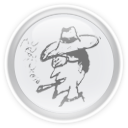
\includegraphics[width=18mm]{agent_white}
  }}
\caption{Estate agent}
\label{agent}
\end{figure}

\begin{figure}[h]
  \centerline{\hbox{
    
\includegraphics[width=135mm]{flat_hunters_white}
  }}
\caption{Flat hunters}
\label{hunters}
\end{figure}

  \section{Getting Started}
    \emph{What you need for running \emph{Flat Hunt}\ldots}

\subsection{Required Libraries}
\subsection{Download}
\subsection{Installation}

  \section{Gameplay}
    \emph{Playing Flat Hunt is not very difficult, especially for those that know the game ``Scotland Yard''\ldots}\\


\subsection{General Rules}
 The game lasts for at most 23 rounds. In these 23 rounds, the flat hunters try to find the estate agent, while he tries to avoid them (this is because he would rather rent the flats to elderly couples, since presumably they make fewer parties in the middle of the night\ldots).\\

In each round, every player can make one move on the public transport system. The estate agent is the first, then it's the hunters' turn. One move is either 

\begin{itemize}
  \item  one or two stops by tram (colored lines),
  \item  one stop by train (thick orange lines),
  \item  or one stop by bus (thin light blue lines).
\end{itemize}

A move with a certain transport can only be made if one has still enough tickets (see \autoref{ticket_status}), if there is a connection (obviously), and if there is no other player at that destination (and in the case of tram lines, if there is no hunter in between).\\

 \textcolor{red}{Attention: If you are at a bus-only stop, and you run out of bus tickets, you will get stuck there forever, so be careful\ldots}\\

\begin{figure}[h]
  \centerline{\hbox{
    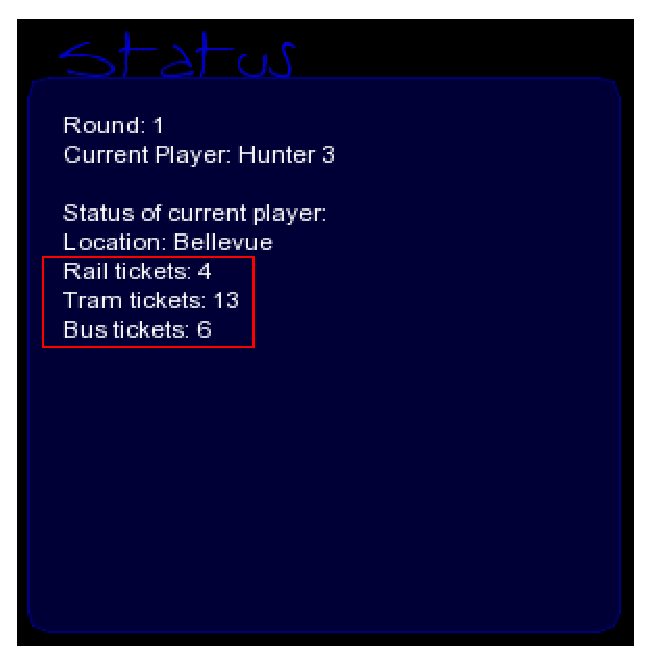
\includegraphics[width=50mm]{ticket_status}
  }}
\caption{Ticket status}
\label{ticket_status}
\end{figure}

The possible places you can move to are colored yellow (see \autoref{highlighted_places}). To make a move, just click on one of those highlighted places. The red circle centers on the player whose turn it is, and in the status box at the right, the game status and information about the current player get displayed. If you want to know the status of another player just click on his picture at the bottom. Click again to close the just opened status box.\\

\begin{figure}[h]
  \centerline{\hbox{
    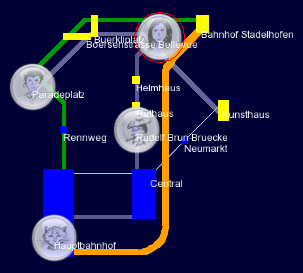
\includegraphics[width=50mm]{highlighted_places}
  }}
\caption{Highlighted places}
\label{highlighted_places}
\end{figure}

The game is over when

  \begin{description}
    \item[a)]the hunters could not find the estate agent within 23 rounds,
    \item[b)]one flat hunter moves onto the place where the agent currently is,
    \item[c)]or the hunters encircle the estate agent so that he cannot move anymore.
  \end{description}

In case a), the winner is the estate agent (he does not have to rent his flat to students), whereas in b) and c) it is the hunters that win, as they get to meet the estate agent on time and thus manage to find a flat.


\subsection{\label{game_modes}Game Modes}
There are four modes to play \emph{Flat Hunt}: \emph{Hunt}, \emph{Escape}, \emph{Versus} and \emph{Demo}. Depending on the mode, zero (\emph{Versus}), one (\emph{Hunt/Escape}) or two (\emph{Demo}) parts are taken over by the computer.

  \begin{description}
    
    \item[Hunt]This is probably the most typical situation; the player tries to find the agent, which is played by the computer. Thus, the player only knows about every fifth move where the agent just was\ldots The agent shows himself only in rounds number 1, 3, 8, 13, 18, and 23. In these rounds, the exact route of the agent is displayed under \emph{History} in the status box at the bottom right corner and in the estate agent's own status box if opened. In all other rounds you only see the detailed history up to the round the estate agent last showed himself. As soon as the agent has come out of hiding for the first time, a dimmed version of his picture will always be shown at the location he was last sighted.

    \item[Escape]This is the exact opposite of \emph{Hunt} mode: The agent is played by you, and the hunters are played by the computer. The hunters always move as close in your direction as possible, as they somehow manage to decode your transponder signal, and thus always know your precise location (so much for privacy\ldots). You just have to try to avoid them as long as possible\ldots
  
    \item[Versus]This is the multiplayer mode. One of the players is the agent; the other plays all the hunters. While the player of the agent is making a move, the player of the hunters is supposed to look away\ldots
   
    \item[Demo]This mode is more or less the opposite of the buzzword ``interactive'', but is about as entertaining as watching fish in an aquarium. The computer is playing against himself, trying to catch the agent as fast as possible.
  
  \end{description}

\subsection{Other}
  When you run \emph{Flat Hunt}, the first you'll see is a menu (see Figure 7). You can either let the default options in place and just select \emph{start game} or you can adjust the settings to your needs. \emph{Game mode} is explained in \ref{game_modes} Game Modes, \emph{number of hunters} and \emph{map size} should be self-explanatory and \emph{characters} specifies which pictures to use for the players. To toggle between the settings menu and the normal menu press \emph{tab}.\\

  During the game when you press \emph{p}, the pause menu is shown. \emph{Continue} makes the pause menu disappear and lets you resume the game, \emph{new game} takes you to the start menu and \emph{quit} quits the application.\\

  The game over menu is similar to the pause menu, only there is no \emph{continue} in this one.


 
  \section{Special Features}
    \subsection{Map Control}
Map control is fairly simple: you got two maps in a game scene, one of which only is a smaller version of the other one. The big map is on the left and that's where the action takes place, the little map on the right is meerely a navigation tool. To control the big map, use your mouse as follows:

  \begin{description}
    \item[left click:] only has an impact if clicked on a highlighted place
    \item[richt click + move mouse:] moves map in the direction of your mouse movement
    \item[middle click + move mouse up:] zoom in
    \item[middle click + move mouse down:] zoom out
  \end{description}

  When you \emph{left click + move mouse} in the little map, a light green rectangle is drawn between the point where your left mouse button is pressed down and the point when its released. As soon as you release the mouse button, the map segment that is inside this rectangle gets displayed on the big map.
 
\subsection{Music Player}
\emph{Flat Hunt} comes with an integrated music player and some default background music. Since not everyone likes the same sound, there is also the possibility to play your own.\\ 
Just put your \texttt{.ogg}-files in the directory \texttt{\$\{FLAT\_HUNT\}/resources/sound} before you start the Flat Hunt application. Flat Hunt will then automatically load all the \texttt{.ogg}-files from this directory and play them in alphabetical order (unless you enable shuffle, obviously). Music player control: see \ref{shortcuts} Keyboard Shortcuts.

\subsection{\label{shortcuts}Keyboard Shortcuts}

During the game, the following shortcuts are available:

  \begin{description}
    \item[p:] pause the game and show pause menu
    \item[s:] music player toggle shuffle
    \item[v:] music player decrease volume
    \item[shift + v:] music player increase volume (at startup the volume is already at maximum)
    \item[page up:] music player next song
    \item[page down:] music player previous song
    \item[q:] quit the application
  \end{description}

  \section{Legal Stuff and Thanks}
    This document is based upon its prior version, which was written by Michela Pedroni and Marcel Kessler (thanks!). All graphics for the game were designed by me and Photoshop. The code of \emph{Flat Hunt} is based on its prior version \cite{mk04}, which is mainly the work of Marcel Kessler. Major parts had to be rewritten by me though.\\

Thanks to Michela Pedroni for her assistance, all my predecessors for their work, Till G. Bay (and others) for the \emph{EiffelMedia} Library (formerly \emph{ESDL} \cite{tgb03}\cite{bb04}) and Bertrand Meyer for the \emph{Eiffel} language. 


    
    \pdfbookmark[1]{References}{ugref}
    \hyperref[ugref]{}    
    \begin{thebibliography}{150}

  \bibitem{bm03} Bertrand Meyer. \emph{The Outside-In Method of Teaching Introductory Programming}. 2003.\\
    \url{http://www.inf.ethz.ch/~meyer/publications/teaching/teaching-psi.pdf}

  \bibitem{mp03} Michela Pedroni. \emph{Teaching Introductory Programming with the Inverted Curriculum Approach}. ETH Zurich, 2003.\\
    \url{http://se.inf.ethz.ch/projects/michela\_pedroni}
    
  \bibitem{rk05} Roger K�ng. \emph{Touch User Guide}. ETH Zurich, 2005.\\
    \url{http://se.inf.ethz.ch/projects/roger\_kueng}
    
  \bibitem{sa05} Sibylle Aregger. \emph{Redesign of the TRAFFIC library}. ETH Zurich, 2005.\\
    \url{http://se.inf.ethz.ch/projects/sibylle\_aregger}
    
  \bibitem{rb05} Rolf Bruderer. \emph{Object-Oriented Framework for Teaching Introductory Programming}. ETH Zurich, 2005.\\
    \url{http://se.inf.ethz.ch/projects/rolf\_bruderer}
    
  \bibitem{mk04} Marcel Kessler. \emph{Exercise Design for Introductory Programming. "Learn-by-doing" basic OO-concepts using Inverted Curriculum}. ETH Zurich, 2004.\\
    \url{http://se.inf.ethz.ch/projects/marcel\_kessler}

  \bibitem{bb04} Benno Baumgartner. \emph{ESDL - Eiffel Simple Direct Media Library}. ETH Zurich, 2004.\\
    \url{http://se.inf.ethz.ch/projects/benno\_baumgartner}
    
  \bibitem{tgb03} Till G. Bay. \emph{Eiffel SDL Multimedia Library (ESDL)}. ETH Zurich, 2003.\\
    \url{http://se.inf.ethz.ch/projects/till\_bay}

\end{thebibliography}
    

    
\end{document}
